\documentclass[paper=letter,11pt]{scrartcl}

\KOMAoptions{headinclude=true, footinclude=false}
\KOMAoptions{DIV=14, BCOR=5mm}
\KOMAoptions{numbers=noendperiod}
\KOMAoptions{parskip=half}
\addtokomafont{disposition}{\rmfamily}
\addtokomafont{part}{\LARGE}
\addtokomafont{descriptionlabel}{\rmfamily}
%\setkomafont{pageheadfoot}{\normalsize\sffamily}
\setkomafont{pagehead}{\normalsize\rmfamily}
%\setkomafont{publishers}{\normalsize\rmfamily}
\setkomafont{caption}{\normalfont\small}
\setcapindent{0pt}
\deffootnote[1em]{1em}{1em}{\textsuperscript{\thefootnotemark}\ }


\usepackage{amsmath}
\usepackage[varg]{txfonts}
\usepackage[T1]{fontenc}
\usepackage{graphicx}
\usepackage{xcolor}
\usepackage[american]{babel}
% hyperref is needed in many places, so include it here
\usepackage{hyperref}

\usepackage{xspace}
\usepackage{multirow}
\usepackage{float}


\usepackage{braket}
\usepackage{bbm}
\usepackage{relsize}
\usepackage{tcolorbox}

\def\ketY{\ensuremath{\ket {\Psi}}}
\def\iGeV{\ensuremath{\textrm{GeV}^{-1}}}
%\def\mp{\ensuremath{m_{\textrm{proton}}}}
\def\rp{\ensuremath{r_{\textrm{proton}}}}
\def\me{\ensuremath{m_{\textrm{electron}}}}
\def\aG{\ensuremath{\alpha_G}}
\def\rAtom{\ensuremath{r_{\textrm{atom}}}}
\def\rNucl{\ensuremath{r_{\textrm{nucleus}}}}
\def\GN{\ensuremath{\textrm{G}_\textrm{N}}}
\def\ketX{\ensuremath{\ket{\vec{x}}}}
\def\ve{\ensuremath{\vec{\epsilon}}}


\def\ABCDMatrix{\ensuremath{\begin{pmatrix} A &  B  \\ C  & D \end{pmatrix}}}
\def\xyprime{\ensuremath{\begin{pmatrix} x' \\ y' \end{pmatrix}}}
\def\xyprimeT{\ensuremath{\begin{pmatrix} x' &  y' \end{pmatrix}}}
\def\xy{\ensuremath{\begin{pmatrix} x \\ y \end{pmatrix}}}
\def\xyT{\ensuremath{\begin{pmatrix} x & y \end{pmatrix}}}

\def\IMatrix{\ensuremath{\begin{pmatrix} 0 &  1  \\ -1  & 0 \end{pmatrix}}}
\def\IBoostMatrix{\ensuremath{\begin{pmatrix} 0 &  1  \\ 1  & 0 \end{pmatrix}}}
\def\JThree{\ensuremath{\begin{pmatrix}    0 & -i & 0  \\ i & 0  & 0 \\ 0 & 0 & 0 \end{pmatrix}}} 
\def\JTwo{\ensuremath{\begin{bmatrix}    0 & 0 & -i  \\ 0 & 0  & 0 \\ i & 0 & 0 \end{bmatrix}}}
\def\JOne{\ensuremath{\begin{bmatrix}    0 & 0 & 0  \\ 0 & 0  & -i \\ 0 & i & 0 \end{bmatrix}}}
\def\etamn{\ensuremath{\eta_{\mu\nu}}}
\def\Lmn{\ensuremath{\Lambda^\mu_\nu}}
\def\dmn{\ensuremath{\delta^\mu_\nu}}
\def\wmn{\ensuremath{\omega^\mu_\nu}}
\def\be{\begin{equation*}}
\def\ee{\end{equation*}}
\def\bea{\begin{eqnarray*}}
\def\eea{\end{eqnarray*}}
\def\bi{\begin{itemize}}
\def\ei{\end{itemize}}
\def\fmn{\ensuremath{F_{\mu\nu}}}
\def\fMN{\ensuremath{F^{\mu\nu}}}
\def\bc{\begin{center}}
\def\ec{\end{center}}
\def\nus{$\nu$s}

\def\adagger{\ensuremath{a_{p\sigma}^\dagger}}
\def\lineacross{\noindent\rule{\textwidth}{1pt}}

\newcommand{\multiline}[1] {
\begin{tabular} {|l}
#1
\end{tabular}
}

\newcommand{\multilineNoLine}[1] {
\begin{tabular} {l}
#1
\end{tabular}
}



\newcommand{\lineTwo}[2] {
\begin{tabular} {|l}
#1 \\
#2
\end{tabular}
}

\newcommand{\rmt}[1] {
\textrm{#1}
}


%
% Units
%
\def\m{\ensuremath{\rmt{m}}}
\def\GeV{\ensuremath{\rmt{GeV}}}
\def\pt{\ensuremath{p_\rmt{T}}}


\def\parity{\ensuremath{\mathcal{P}}}

\usepackage{cancel}
\usepackage{ mathrsfs }
\def\bigL{\ensuremath{\mathscr{L}}}

\usepackage{ dsfont }



\usepackage{fancyhdr}
\fancyhf{}

\usepackage{braket}

\def\ketY{\ensuremath{\ket {\Psi}}}
\def\iGeV{\ensuremath{\textrm{GeV}^{-1}}}
\def\mp{\ensuremath{m_{\textrm{proton}}}}
\def\rp{\ensuremath{r_{\textrm{proton}}}}
\def\me{\ensuremath{m_{\textrm{electron}}}}
\def\aG{\ensuremath{\alpha_G}}
\def\rAtom{\ensuremath{r_{\textrm{atom}}}}
\def\rNucl{\ensuremath{r_{\textrm{nucleus}}}}
\def\GN{\ensuremath{\textrm{G}_\textrm{N}}}

\def\be{\begin{equation*}}
\def\ee{\end{equation*}}


\usepackage{fancyhdr}
\usepackage{cancel}
\usepackage{ mathrsfs }





\fancyhf{}
\lhead{\Large 33-444} % \hfill Introduction to Particle Physics \hfill Spring 2019}
\chead{\Large Introduction to Particle Physics} % \hfill Spring 2019}
\rhead{\Large Spring 2019} % \hfill Introduction to Particle Physics \hfill Spring 2019}
\begin{document}
\thispagestyle{fancy}





%\begin{tabular}{c}
%{\large 33-444 \hfill Intro To Particle \hfill Spring 2019\\}
%\hline 
%\end{tabular}

\begin{center}
{\huge \textbf{Homework Set \#5}}
\large

{\textbf{ Due Date:} Before class Friday February 22nd  } 
\end{center}

{\large
\textbf{1) Clifford Algebra \hfill \textit{(5 points)} }

In writing the Dirac equation, we chose a particular representation of the $\gamma$ matrices that satisfied $\{\gamma_\mu,\gamma_\nu\} = 2\eta_{\mu\nu}$, which is called the Clifford algebra. 
The choice we used in class is called the Weyl basis. In this problem, we will study the Clifford algebra and the Weyl basis.
\begin{itemize}
\item[a)]
By explicit multiplication, show that the $\gamma$ matrices in the Weyl basis satisfy the Clifford algebra.
\item[b)]
The Weyl basis isn’t the unique choice of matrices that satisfy the Clifford algebra. 
Another set of matrices that does is
\begin{equation*}
\gamma_0 = \begin{pmatrix} I &  0 \\ 0 & -I \end{pmatrix} \hspace{0.5in} \gamma_i = \begin{pmatrix} 0 & \sigma_i \\  -\sigma_i & 0 \end{pmatrix}
\end{equation*}
This choice of $\gamma$ matrices is related to the Weyl basis by a similarity transformation:
\begin{equation*}
\gamma_\mu = S\gamma_\mu^{\mathrm{Weyl}}S^\dagger, 
\end{equation*}
where S is a unitary matrix such that $SS^\dagger = I$.
A similarity transformation of the $\gamma$ matrices respects the Clifford algebra. 
Determine the matrix S that relates the Weyl basis to this new basis of $\gamma$ matrices.

\item[c)]
 Applying the similarity transformation to the Dirac equation, gives 
\begin{equation*}
(i S \gamma_\mu S^\dagger \partial^{\mu} - m)\psi = S(i\gamma \cdot \partial - m)S^\dagger\psi = 0.
\end{equation*}
Given the solution to the Dirac equation that we found in class, use the similarity transformation S you found above part to find the solutions to the Dirac equation using the $\gamma$ matrix in the new basis.
\end{itemize}

\vspace*{0.25in}

\textbf{2) Show that  $\mathscr{L}_{EM} = -\frac{1}{4}F_{\mu\nu}F^{\mu\nu} - J^{\mu}A_{\mu}$ is gauge invariant \hfill \textit{(5 points)}}


\vspace*{0.25in}


%\begin{itemize}
%\item[] { }
%\end{itemize}


\textbf{3) Maxwell’s Equations.\hfill \textit{(5 points)}}
\begin{itemize}
\item[a)]In class,  I mentioned  that Gauss’s law follows from taking the 0 component of the equations of motion of the electromagnetic Lagrangian $\partial_\mu F^{\mu\nu} = J^\nu$. 
Show this explicitly.
\item[b)]Show that the three other of Maxwell’s equations follow from the equations of motion and the Bianchi identity ($\partial_\mu F_{\nu\rho} +\partial_\rho F_{\mu\nu} +\partial_\nu F_{\rho\mu} =0$). \textit{Hint: take individual components and identify the corresponding Maxwell’s equation.}
\end{itemize}

\vspace*{0.25in}

\textbf{4) Lagrangians.\hfill \textit{(5 points)}}
\begin{itemize}
\item[a)]The celebrated Euler-Lagrange equations give the equations of motion following from a Lagrangian. 
They are: 
\be
\frac{\partial \mathscr{L}}{\partial \phi} - \partial_\mu \frac{\partial \mathscr{L}}{\partial(\partial_\mu \phi)} = 0.
\ee
Derive the Euler-Lagrange equations from setting the variation of action with respect to $\phi$ and $\partial_\mu phi$  to 0.
\item[b)]Show that the Klien Gordon equation is the equation of motion associated with the Lagrangian:f $\mathscr{L}= \frac{1}{2}(\partial_\mu \phi)(\partial^{\mu}\phi) = \frac{1}{2}m^2\phi^2$
\item[b)]What is the Noether's current associated to the continuous symmetry $\phi \rightarrow e^{-i\alpha} \phi$ of the Lagrangian $\mathscr{L}= \frac{1}{2}(\partial_\mu \phi)(\partial^{\mu}\phi^*) - \frac{1}{2}m^2\phi\phi^*$
\end{itemize}

\vspace*{0.25in}

\textbf{5) Dark Matter Searches. \hfill \textit{(10 points)}}

Numerous experiments are searching for dark matter, a component of energy in the universe necessary for the observed features of early universe cosmology, large-scale structure, and galactic dynamics. 
There has been no direct evidence for a particle nature of dark matter as of yet, but there are very strong constraints on its properties. 
Some of the strongest constraints were imposed by null observations of the LUX (Large Underground Xenon) dark matter experiment. 
LUX consists of a vat of 250 kg of ultra-pure liquid xenon situated about one mile underground in the Sanford Underground Research Facility in Lead, South Dakota. 
For this problem, assume that the xenon is pure $^{131}$Xe.

A major result from the LUX experiment is shown in the figure below. 
This is a plot of the constraints that it has placed on possible dark matter particles called WIMPs (Weakly Interacting Massive Particles). 
LUX searches for WIMPs by their scattering off of the $^{131}$Xe nuclei. 
If a significant amount of kinetic energy is transferred to the $^{131}$Xe, then it excites a scintillator and is observed as a ``hit.''
The amount of kinetic energy transfer is a function of the WIMP mass (shown on the x-axis on the plot) and the rate of hits is a function of the strength of interaction of the WIMPs with xenon (the y-axis on the plot). 
The interaction strength is measured in a unit of cross section called zeptobarns.
We’ll introduce the ``barn'' unit next week. 


\begin{figure}[h]
\centering
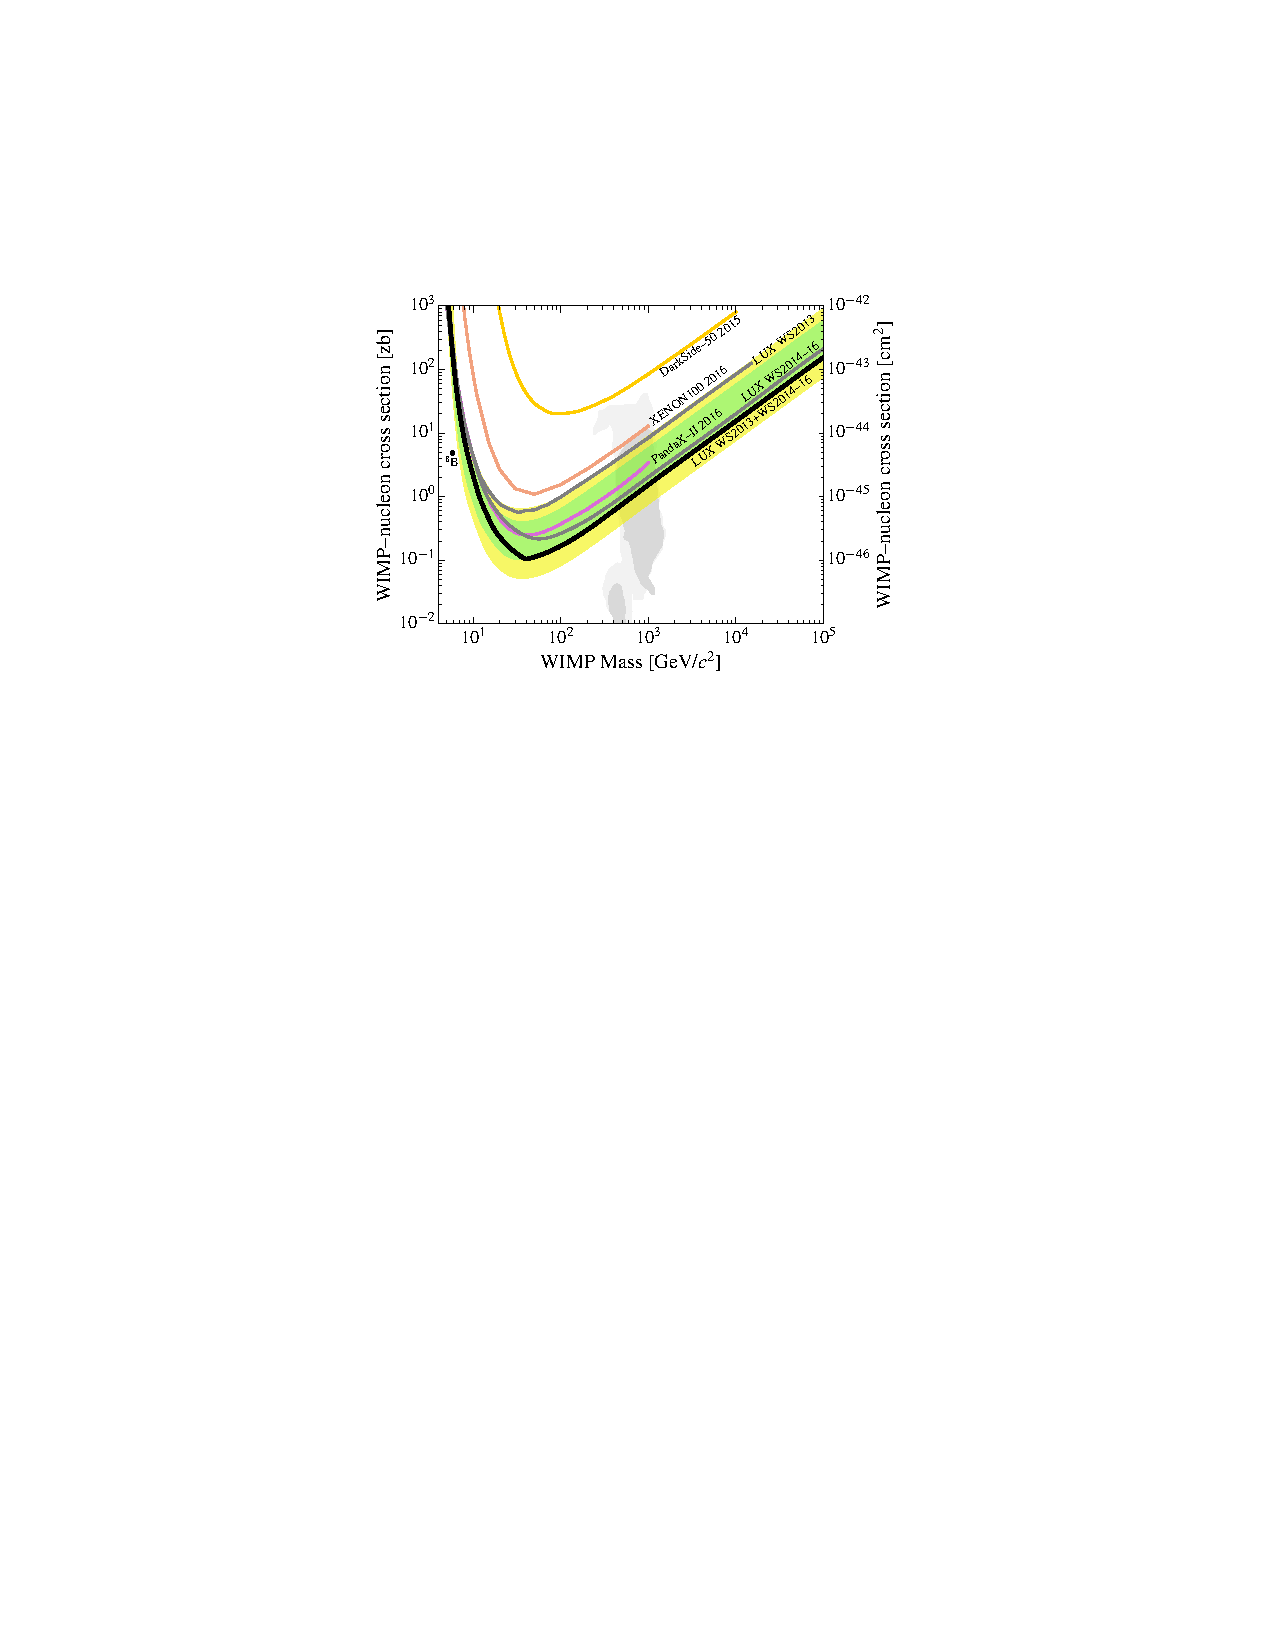
\includegraphics[width=0.6\textwidth]{./LuxLimits.pdf}
\caption{A plot of the WIMP mass and interaction strength limits from the LUX experiment. From D. S. Akerib et al. [LUX Collaboration], “Results from a search for dark matter in the complete LUX exposure,” Phys. Rev. Lett. 118, no. 2, 021303 (2017) arXiv:1608.07648].
}
\end{figure}


WIMP masses and interaction strengths have been ruled out (i.e., observed to not exist) by the LUX experiment above the thick black curve. 
In this exercise, we will study where the lower bound on the WIMP mass comes from (the nearly vertical bound on the left of the plot).
We will come back to the bound on higher masses in a later problem set. 

\begin{itemize}
\item[a)]
A model for WIMP dark matter in the MilkyWay galaxy is as a spherically-distributed halo of particles that is at rest. 
How fast is the WIMP’s apparent speed through the LUX detector on Earth? 
The radius of the solar system’s orbit around Milky Way is about 25,000 light years with an orbital period of about 230,000,000 years. 
(The fact that the Earth orbits the Sun affects this on a yearly timescale, but we will ignore this small effect.)
\item[b)]
The scattering process that LUX is sensitive to is
\begin{equation*}
\chi + \mathrm{^{131}Xe} \rightarrow \chi + \mathrm{^{131}Xe}
\end{equation*}
where $\chi$ denotes a WIMP particle. 
Write down the four-vectors for all particles involved in this collision. 
Assume that the initial xenon nucleus is at rest, and the initial dark matter particle $\chi$’s momentum is aligned along the z axis. 
Call these four-vectors $p_{Xe}$ and $p_\chi$, respectively. 
After collision, assume that both $\chi$ and xenon only have a non-zero z component of momentum. 
Call the four-vectors after collision $p'_\chi$ and $p'_{\mathrm{Xe}}$. 
Make sure all four-vectors are on-shell and enforce three-momentum conservation (don’t worry about energy conservation yet). 
Express the four vectors in terms of the mass of the WIMP m$\chi$, the mass of the xenon nucleus $m_{\mathrm{Xe}}$, the initial z momentum of the WIMP $p_z$, and the final z component of momentum of the xenon, $p^{\mathrm{Xe}}_z$. 
(Assuming that the scattering occurs in a line means that the energy transfer to the xenon is maximized.)
\item[c)]
Using the conservation of the momentum four-vectors, solve for the recoiling xenon’s momentum $p^{\mathrm{Xe}}_z$.
(\textit{Hint:} A nice way to do this is to write $p^{\mathrm{Xe}}_z = \alpha p_z$ and solve for $\alpha$).
You should find two solutions. 
What is the solution corresponding to the larger value of momentum?
\item[d)]
LUX measures the recoiling xenon nucleus’s kinetic energy K. 
Relativistically, this is defined as $K = E-m_{\mathrm{Xe}}$. 
What is the kinetic energy of the recoiling xenon nucleus as a function of WIMP mass $m_\chi$ and momentum $p_z$? 
Because the velocity of the dark matter halo is small, Taylor expand your result to lowest non-zero order in $p_z$ and set $p_z = m\chi v$, where v is the WIMP velocity with respect to Earth.

\item[e)]
Below a kinetic energy of about 1 keV, LUX cannot detect the recoiling xenon nucleus. 
Using the result of the previous part of this problem, what is the minimum dark matter mass that can provide this kinetic energy kick? 
(\textit{Hint:}You’ll also need the WIMP velocity v calculated in part (a) of this problem. )
Compare this mass to the lower mass bound in the figure. 
%(We’ve made many simplifications, so you should see that LUX is sensitive to masses a bit below what you will find in this problem.)

\end{itemize}
 




}





\end{document}
